\chapter{Describing Data Sets}

\section{Data Sets}

  \begin{itemize}
    \item A data set $ \{ x \} $ is a collection of items $ x_{1}, x_{2} ... x_{n} $;
    \item Each item in the data set can be a tuple;
  \end{itemize}
  
\section{Types of Data}

  \begin{itemize}
    \item \textbf{Categorical}: a small set of set values;
    \item \textbf{Ordinal}: values that can be ordered;
    \item \textbf{Continuous}: values that fall into a range;
  \end{itemize}
  
\section{Summarizing Data}

  \begin{itemize}
    \item \textbf{Mean and standard deviation} are very sensitive to outliers;
    \item \textbf{Median and interquartile range} are not sensitive to outliers;
  \end{itemize}

  \subsection{Mean}
  
    \begin{equation}
      \mean \left( \{ x \} \right) = \frac{1}{N} \sum_{i=1}^{N} x_{i}
    \end{equation}
    
    \subsubsection{Properties}
    
      \begin{enumerate}
        \item Scaling data sclaes the mean;
        \begin{equation}
          \mean \left( \{ k \times x_{i} \} \right) = k \times \mean \left( \{ x_{i} \} \right)
        \end{equation}

        \item Translating the data translates the mean;
        \begin{equation}
          \mean \left( \{ x_{i} + c \} \right) = \mean \left( \{ x_{i} \} \right) + c
        \end{equation}
        
        \item Sum of signed distance from mean is 0:
        \begin{equation}
          \sum_{i = 1}^{N} \left( x_{i} - \mean \left( \{ x \} \right) \right) = 0
        \end{equation}
        
        \item Let $ \mu $ be a point. The sum of data points to $ \mu $ is minimized. The data point is the mean;
      \end{enumerate}

  \subsection{Standard Deviation}
  
    \begin{equation}
      \std\left( \{ x \} \right) = \sqrt{ \frac{1}{N} \sum_{i = 1}^{N} \left[ x_{i} - \mean\left( \{ x \} \right) \right]^{2} }
    \end{equation}
    
    \subsubsection{Properties of Standard Deviation}
    
      \begin{enumerate}
        \item Scaling the data scales the standard deviation:
        \begin{equation}
          \std\left( \{ kx \} \right) = \left| k \right| \std\left( \{ x \} \right)
        \end{equation}
        
        \item Translating the data \textbf{does NOT translate the standard deviation}
        \begin{equation}
          \std\left( \{ x_{i} + c \} \right) = \std\left( \{ x \} \right)
        \end{equation}
        
        \item Given a data set with $ N $ items, there can be at most $ \dfrac{N}{k^{2}} $ items that are $ k $ items away from the mean;
      \end{enumerate}
      
  \subsection{Variance}
  
    \begin{align}
      \var\left( \{ x \} \right) &= \frac{1}{N} \sum_{i = 1}^{N} \left[ x_{i} - \mean\left( \{ x \} \right) \right]^{2} \\
      &= \std\left( \{ x \} \right)^{2}
    \end{align}
    
    \begin{enumerate}
      \item Scaling data scales the variance;
      \begin{equation}
        \var \left( \{ k \times x_{i} \} \right) = k^{2} \times \var \left( \{ x_{i} \} \right)
      \end{equation}

      \item Translating the data \textbf{does NOT influence the variance}
      \begin{equation}
        \var \left( \{ x_{i} + c \} \right) = \var \left( \{ x_{i} \} \right)
      \end{equation}
    \end{enumerate}
    
  \subsection{Median}
      
    \begin{itemize}
      \item In a sorted set:
      \begin{itemize}
        \item the \textbf{median is the middle item, if there are an odd number of items};
        \item the \textbf{median is the mean of middle two items if there are an even number of items};
      \end{itemize}
      
      \item Also known as the \textbf{50th percentile};
    \end{itemize}
    
    \subsubsection{Properties}
    
      \begin{enumerate}
        \item Scaling the data scales the median:
        \begin{equation}
          \median \left( \{ k \times x_{i} \} \right) = k \times \median \left( \{ x_{i} \} \right)
        \end{equation}

        \item Translating the data translates the median:
        \begin{equation}
          \median \left( \{ x_{i} + c \} \right) = \median \left( \{ x_{i} \} \right) + c
        \end{equation}
      \end{enumerate}
      
  \subsection{Interquartile Range}
  
    \subsubsection{Definitions}
    
      \begin{itemize}
        \item \textbf{Percentile}: the k'th percentile is a value such that $ k \% $ of hte data is less than or equal to that value.
        \begin{itemize}
          \item $ \percentile\left( \{ x \}, k \right) $ is hte k'th percentile of the dataset $ \{ x \} $;
        \end{itemize}
        
        \item \textbf{Quartiles}: 
        \begin{itemize}
          \item \textbf{First quartile}: $ \percentile\left( \{ x \}, 25 \right) $;
          \item \textbf{Second quartile}: $ \percentile\left( \{ x \}, 50 \right) $;
          \item \textbf{Third quartile}: $ \percentile\left( \{ x \}, 75 \right) $;
        \end{itemize}
        
        \item \textbf{Interquartile Rnage}: the interquartile range $ \iqr $ is the third percentile minus the first percentile
        \begin{equation}
          \iqr\{ x \} = \percentile\left( \{ x \}, 75 \right) - \percentile\left( \{ x \}, 25 \right)
        \end{equation}
        \begin{itemize}
          \item Interquartile range \textbf{describes the scale of data}, but is \textbf{less affected by outliers};
        \end{itemize}
      \end{itemize}
      
    \subsubsection{Properties}
    
      \begin{itemize}
        \item Scaling the data scales the interquartile range;
        \begin{equation}
          \iqr \left( \{ k \times x_{i} \} \right) = \left| k \right| \times \iqr \left( \{ x_{i} \} \right)
        \end{equation}
        
        \item Translating the data \textbf{does NOT translates the interquartile range};
        \begin{equation}
          \iqr \left( \{ x_{i} + c \} \right) = \iqr \left( \{ x_{i} \} \right)
        \end{equation}
      \end{itemize}
    
\section{Plot}

  \subsection{Standard Coordinates}
  
    \begin{equation}
      \hat{x_{i}} = \frac{ x_{i} - \mean\left( \{ x \} \right) }{ \std \left( \{ x \} \right) }
    \end{equation}
  
    \begin{itemize}
      \item Given a set of data $ \{ x \} $, the standard coordinates of the data is $ \{ \hat{x} \} $;
    \end{itemize}
  
    \paragraph{Why there needs to be standard coordinates}
    \begin{itemize}
      \item Different histograms are in \textbf{different ranges, and different untis}, and thus difficult to compare;
      \item To make the histograms comparable, we need to:
      \begin{enumerate}
        \item Standardize the location of the histograms on the horizontal axis, which is the mean;
        \item Standardize the scale of the histograms, which is the standard deviation;
      \end{enumerate}
      
      \item The location is standardized by subtracting the mean from each coordinate;
      \item The scale is standardized by dividing each coordinate with the standard deviation;
    \end{itemize}
    
    \subsubsection{Properties}
    
      \begin{align}
        \mean\left( \{ \hat{x} \} \right) &= 0 \\
        \std\left( \{ \hat{x} \} \right) &= 1
      \end{align}
      
  \subsection{Histograms}
  
    \begin{itemize}
      \item \textbf{Modes}: peaks in histograms;
      \item \textbf{Tails}: the less high regions to the left and the right of a histogram;
      \item \textbf{Skewed}:
      \begin{itemize}
        \item A histogram is left-skewed if its left tail is significantly longer than the right tail;
        \item A histogram is right skewed if its right tail is significantly longer than the left tail;
      \end{itemize}
    \end{itemize}
    
    \subsubsection{Determine Shape by Comparing Median and Mean}
    
      \begin{tabu} to \linewidth{ X[l] | X[l] }
        \thickhline
        \textbf{Mean vs Median} & \textbf{Shape} \\ \thickhline
        Mean $ > $ Median & Right skewed \\ \hline
        Mean $ < $ Median & Left skewed \\ \hline
        Mean $ = $ Median & Symmetric \\ \hline
      \end{tabu}
      
  \subsection{Box Plots}
  
    \begin{figure}[H]
      \centering
      \caption{Box Plot Composition}
      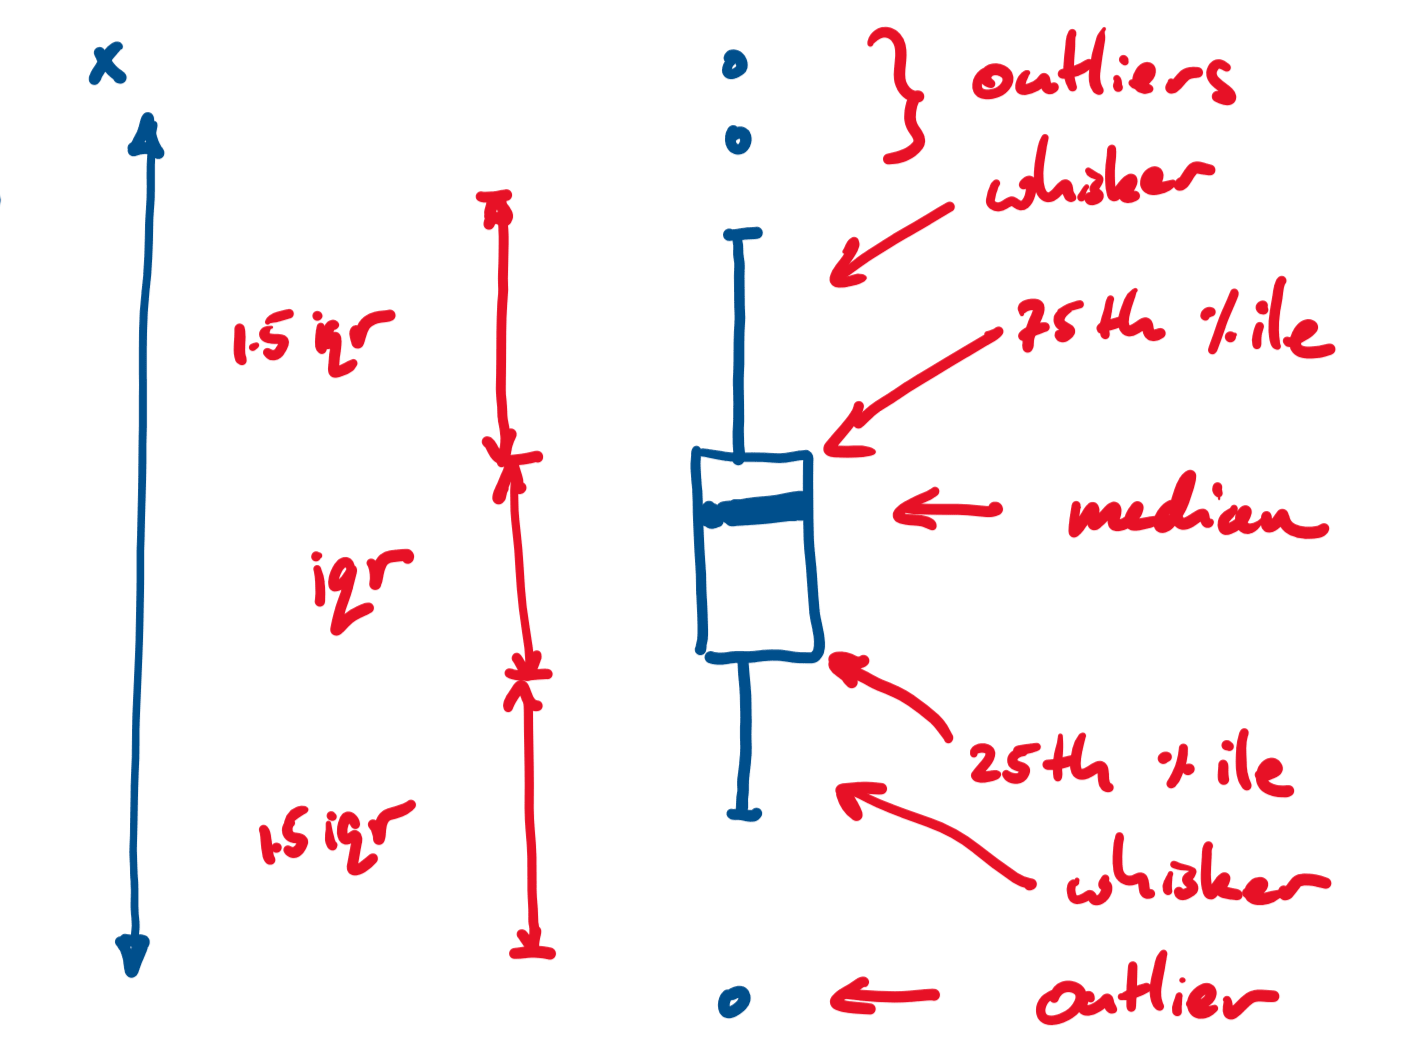
\includegraphics[width=0.7\linewidth]{resources/ch1/box-plot.png}
    \end{figure}